\chapter{Evaluation}
The goal of this paragraph is to assure that the changes we made to AutoWDS basic actually improved its performance.
Due to extent this work is aimed at, it was not feasible to implement all the systems of the related solutions on this field on a common environment
to get a fair assessment for each work. For this the overview papers on this area like \cite{overview_caa} may serve its purpose.
The following subsections will mainly focus on the comparison between AutoWDS basic and the extended version. Also we were not able to evaluate the performance gains
of some metrics like the survival path feature since the current implementation of AutoWDS only uses network bridges to connect the networks and no real routing infrastructure.
Due to this restriction only we are limited to spanning trees for the network since otherwise the STP would force shutdown the redundant links to eliminate
circles in the topology.
\section{Test Arrangement}
Since the main goal is to increase overall throughput performance as described in the requirements analysis, our basic evaluation approach is
to find by how much we were able to increase this metric. Therefore we ran both systems under equal circumstances with various settings and multiple runs
and compared its capacities.
  \subsection{Physical Infrastructure}
    For the test arrangement we used the following hardware:
      11 Accesspoints, 1 WLC and 2 Switches among those
      \begin{itemize}
       \item 3 x Lancom L322agn dual Wireless //cite the website or product catalog?
       \item 3 x Lancom L-452agn dual Wireless
       \item 6 x Hirschmann OpenBAT-R
       \item 1 x Lancom WLC-4100
       \item 2 x Lancom GS-2352P
      \end{itemize}
      running on Firmware Version <<insert version here>>. We deployed them at a typical office environment as depicted in the figure.
      Only omnidirectional antennas for the accesspoints were used for this setup. As we had to connect each of the accesspoints also
      per cable to the monitoring station and power grid in order to route traffic through them and the network they're spanning,
      we could not set them further apart.
      Increasing the distance between the single APs would have lead to a sparser network topology and so the hidden station problem would have occured
      more often. Thus the actual interference would have gone up, since with a lower Signal to Noise ratio the APs would not be able to recognize each others 
      transmissions as those and categorize it as interference instead of applying CSMA/CD, leading to more corrupt packets.
      We were able to simulate this problem with a reduced transmit-power,
      but even on the lowest setting most of the accesspoints were able to receive each others beacons. With this limitation kept in mind we expect
      the gap between the two scenarios in the following results to be even greater.
      Since this test was conducted at a research facility for wireless LAN devices, especially the 2.4Ghz band was quite heavily utilized as you will notice
      in the performance charts.
    \begin{figure}[t]
      \centering
      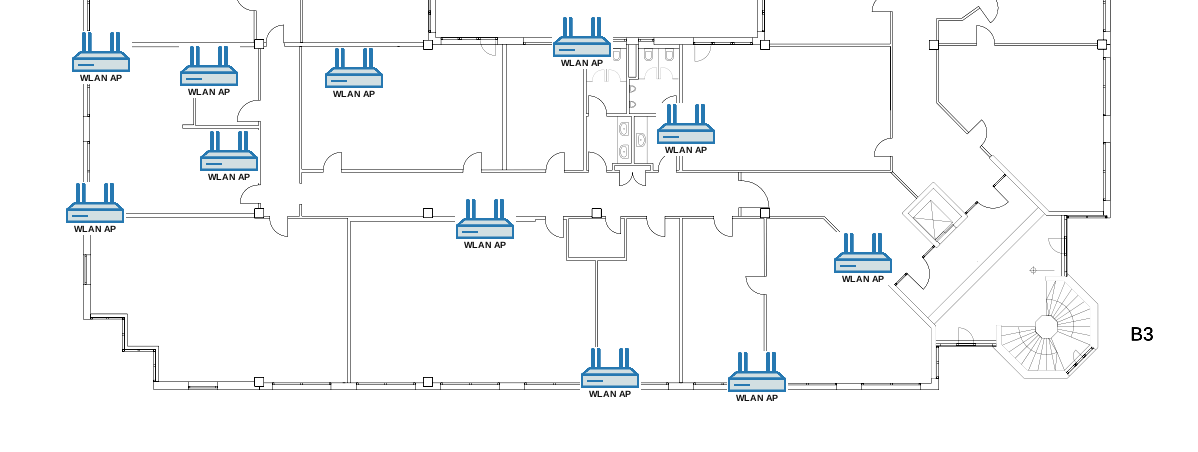
\includegraphics[width=1\columnwidth]{figures/Lancom-flur-withaps}
      \caption{Physical arrangement of accesspoints in a typical office complex spread over an area of rougly 15m x 40m}
      \label{fig:2ndfloor}
    \end{figure}
  \subsection{Network Infrastructure}
    \begin{figure}[h]
      \centerline{
	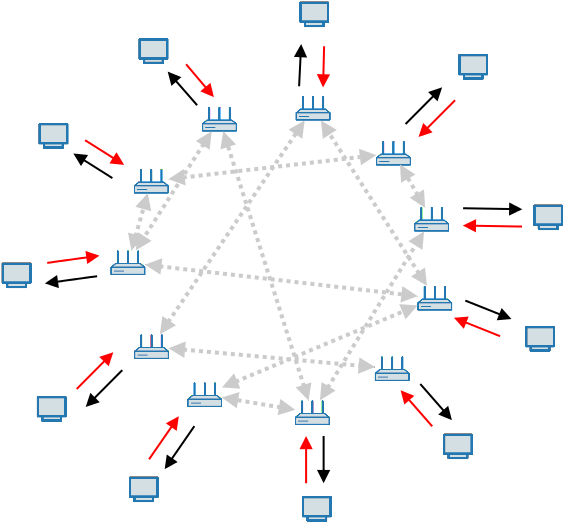
\includegraphics[width=0.3\textwidth]{figures/testsetup_logic}
	\caption{Example for the logical arrangement of accesspoints with systems attached by cable, which generate broadcast traffic that is routed through the 
	wireless network spanned by the accesspoints.}
      }
      \label{fig:testsetup_logic}
    \end{figure}
    The basic approach for measuring the throughput is to attach traffic generators to the accesspoints and make those send as much broadcast traffic to all
    other stations which are part of this network and therefore saturate the throughput capabilities of the network.
    \begin{figure}[h]
      \centerline{
	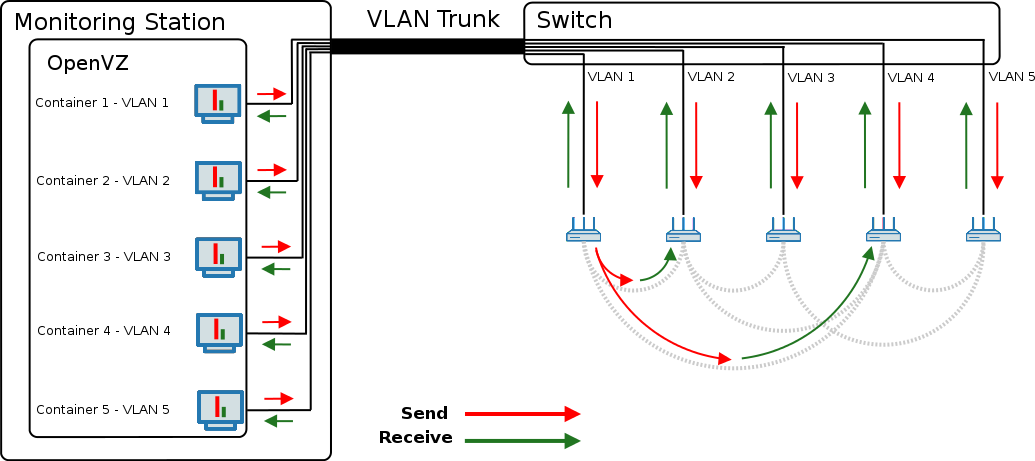
\includegraphics[width=0.6\textwidth]{figures/testsetup_openvz}%
	\caption{Implementation of the test arrangement with available hardware.}
      }
      \label{fig:testsetup_openvz}
    \end{figure}
    We simulated the traffic generating systems with OpenVZ \cite{openvz} on one Host with a VLAN for each system. The VLAN infrstructure is completely transparent
    to the VZ containers and the accesspoints since the monitoring stations encapsulates all frames before sending if over the VLAN Trunk to the switch, which again 
    decapsulates the frames before sending them to the accesspoints.
    To generate the traffic we used IPerf \cite{iperf} on the attached systems in UDP mode with a datarate of 1Mbit per second for a total of 10 Minutes.
    Since we could not directly send UDP frames to broadcast addresses with iperf, we ran multiple instances of iperf with different target ip addresses.
    Although 1Mbit for each stream may not seem much, but after multiplying it with the number of targets and the up- and downstreams the effective rate results in
    1Mbit * 12 * 2 = 24Mbit/s for each accesspoint. As we will see later on this will turn out to be enough to completely saturate the wireless network but still within
    the capabilities of the used Gigabit Ethernet to get the data to the accesspoints, as 24Mbit/s * 11 = 264Mbit/s does not exceed the 1000Mbit/s VLAN Trunk connection
    as possible bottleneck.
    \begin{listing}[t]
      \begin{lstlisting}
iperf -u -c 172.16.40.2* -t 600 -b 1M
      \end{lstlisting}
      \caption{IPerf's parameters to generate the traffic.}
      \label{lst:iperf}
    \end{listing}
\section{Metrics}
  \subsection{Test Duration}
     Each testcase was run for a total of 10 minutes as this should be enough to transgress any temporary effects. To get status snapshots we querried the accesspoints
     every 7 seconds for their state, which includes the bytes transferred and received so far. We did not query them more often since this could have 
     affected the accesspoints transfer performance as reading its internal tables and sending the results back means additional stress.
  \subsection{Channelusage}
    For AutoWDS basic we configured the Accesspoints to only use the following sets of Channels:
    \begin{itemize}
     \item 1 (2.4 GHz only)
     \item 36 (5GHz only)
    \end{itemize}
    For the extended version of AutoWDS we used the following channels as input for the allocation algorithm: 
    \begin{itemize}
     \item 1,6,11 (2.4 GHz only)
     \item 36,40,44 (5GHz only)
     \item 1,6,11,36,40,44 (2.4/5 Ghz mixed)
    \end{itemize}
    
    \begin{figure}[h]
      \centerline{
	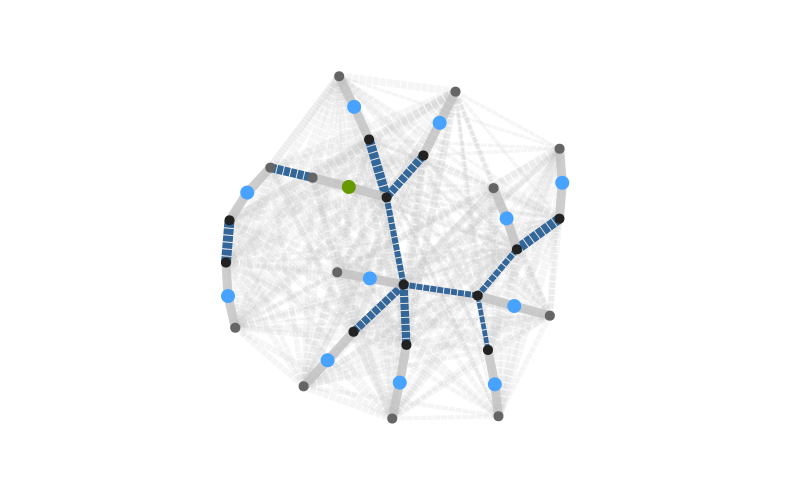
\includegraphics[width=0.7\textwidth]{figures/topo_chan_1}%
	\caption{Topology of the testnetwork with only channel 1 used. Different colors indicate different channels}
      }
      \label{fig:topo_chan_1}
    \end{figure}
    
    \begin{figure}[h]
      \centerline{
	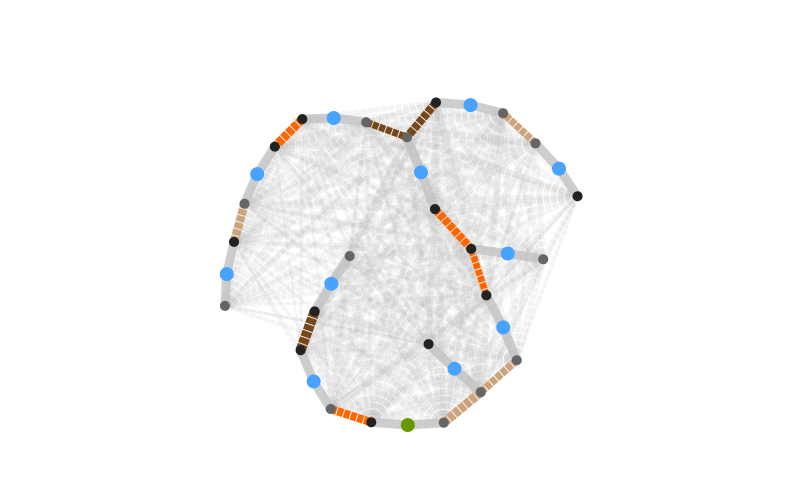
\includegraphics[width=0.7\textwidth]{figures/topo_chan_36_40_44}%
	\caption{Topology of the testnetwork with only channel 36,40,44 being used.}
      }
      \label{fig:topo_chan_36_40_44}
    \end{figure}

    \begin{figure}[h]
      \centerline{
	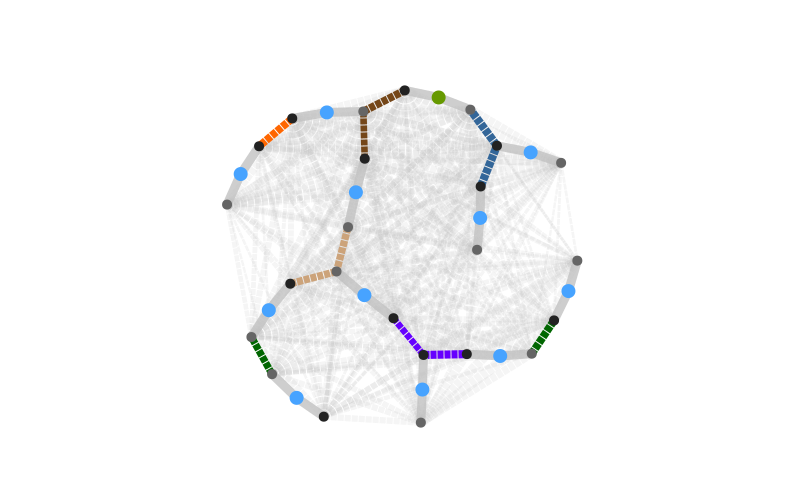
\includegraphics[width=0.7\textwidth]{figures/topo_chan_1_6_11_36_40_44}%
	\caption{Topology of the testnetwork with only channel 1,6,11,36,40,44 being used.}
      }
      \label{fig:topo_chan_1_6_11_36_40_44}
    \end{figure}
    
    \subsection{Characteristics}
    Due to the exceptional utilization of the 2.4 Ghz band in the area around the test arrangement, we had to carefully chose time and day
    for running the tests. We noticed a significant drop in radio usage for weekends and evenings and were able to schedule our tests in those timeframes.
    We additionally ran the testcases with two different settings to simulate the hidden station problem. Therefore we first set the radios to full power 
    resulting in a high connectivity between the nodes and on a second run decreased the transmit power as much as possbile to get a network with a smaller degree
    of interconnectivity.
\section{Results}
  \subsection{Expectations}
    We would expect a significant increase of data that has been able to transmit due to the usage of multiple collision domains the same one could
    expect by comparing a network hub, which has essentially just one collision domain and a network switch which has multiple domains and does not have
    to wait until the medium is free for sending again. The second source for an increased throughput would be the number of packets that could be received
    without errors due to interference.
  \subsection{Actual Results}
    
    \begin{figure}[h]
      \centerline{
	\includegraphics[width=0.62\textwidth]{figures/TestDataDiagramme/20/rx_bytes}%
	\includegraphics[width=0.38\textwidth]{figures/TestDataDiagramme/20/rx_bytes_boxplot}%
	\caption{Received bytes with decreased antenna transmit power}
      }
      \label{fig:rx20_bytes}
    \end{figure}
    
    \begin{figure}[h]
      \centerline{
	\includegraphics[width=0.62\textwidth]{figures/TestDataDiagramme/3/rx_bytes}%
	\includegraphics[width=0.38\textwidth]{figures/TestDataDiagramme/3/rx_bytes_boxplot}%
	\caption{Received bytes with full transmit power}
      }
      \label{fig:rx3_bytes}
    \end{figure}
    
    \begin{figure}[h]
      \centerline{
	\includegraphics[width=0.56\textwidth]{figures/TestDataDiagramme/3/recpackerr}%
	\includegraphics[width=0.44\textwidth]{figures/TestDataDiagramme/3/recpackerr_boxplot}%
	\caption{Ratio of successfully received packets to packets containing errors for reduced transmit power scenario}
      }
      \label{fig:3recpackerr}
    \end{figure}
    
    \begin{figure}[h]
      \centerline{
	\includegraphics[width=0.56\textwidth]{figures/TestDataDiagramme/20/recpackerr}%
	\includegraphics[width=0.44\textwidth]{figures/TestDataDiagramme/20/recpackerr_boxplot}%
	\caption{Ratio of successfully received packets to packets containing errors for full transmit power scenario}
      }
      \label{fig:20recpackerr}
    \end{figure}
    
    The results perfectly match our expectations. They also confirm that the 5Ghz band is superior to the 2.4Ghz with respect to throughput and reliability.
    We used the following channel sets for the actual implementation:
      
    \subsubsection{Assessment of AutoWDS basic}
      Using only a single channel for each wireless link does not scale very well in either of the two power setups, independant of the band used (2.4Gz or 5Ghz).
      Although the 5Ghz channels perform a little better in the high power setup, there seems no recognizable difference for the low power scenario.
      TODO: Explain why 5Ghz better in this scenario.
      Also with an increased transmit-power the number of packets which contain errors increases dramatically from an average of 10 percent to an average of 
      65 percent. TODO: How to explain this?
      Surprisingly the error rates for the 5Ghz channels already start high but seem to increase less than the 2.4Ghz channels.
      The results also affirm our estimate that the current version is not capable of transferring a little more than the control data.
      While setting up our test environment we also noticed that this effect of medium overload is no result of the size of our network.
      Whereas two unimpeded accesspoints were able to achieve a throughput of about 2Mbit in each direction, adding a third one would dramatically 
      decrease overall throughput down to about 100kbit or less, growing worse with each newly added accesspoint in receive-range. Even spreading the 
      accesspoints further apart would not promise better results since the inhering problem of using the same channel for the forwarding and receiving 
      link restricts the forwarding capabilities rigorously.
    \subsubsection{Assessment of AutoWDS extended}
      As the figures show, the outcome is dependent on the number of channels used as a setup with only 3 distinct channels allowed yields still better
      results than a mono-channel-setup but is inferior to a setup where we can use more channels as this gives us the possibility to use more collision domains
      which results in a higher available bandwidth and therefore increased throughput. In our example we used accesspoints with only two radios equipped, which
      limits us in selecting separate modules for different connections so that an accesspoint which already established two connections over its two modules
      would have to share one of its modules in order to apply a new link to a foreign accesspoint in order to maintain connectivity.
      \begin{figure}[h]
	\centerline{
	  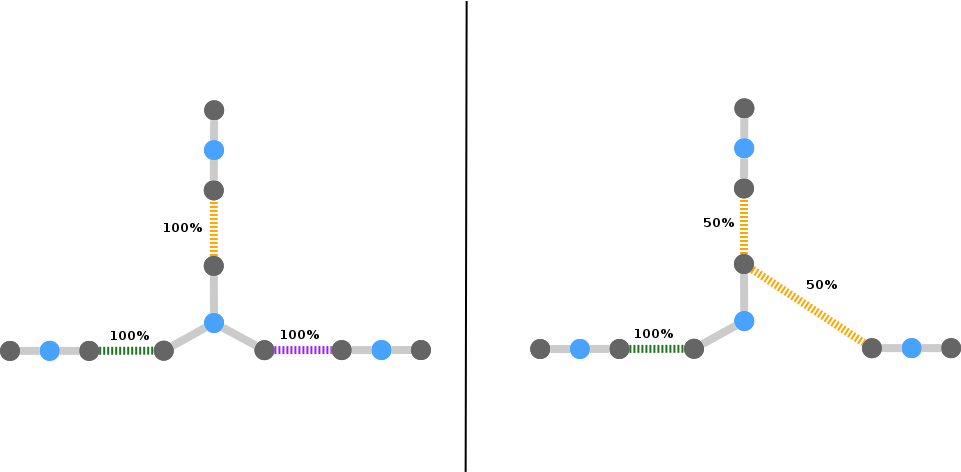
\includegraphics[width=0.56\textwidth]{figures/3modulesvs2}%
	  \caption{Link separation capability for an accesspoint with 3 modules compared to an accesspoints with 2 modules.}
	}
	\label{fig:3modulesvs2}
      \end{figure}
      Compared to the base scenario our link selection and channel assignment algorithm was able to double the throughput with every channel added. Of course this
      effect is limited by using a separate channel for each link and also by the number of modules for an accesspoint 
      since the former effectively assigns each link its own private channel and the latter is a question of practical relevance as current accesspoints are only 
      shipped with 2 or a maximum of 3 radio modules. As our gathered data indicate it is obviously an improvement to utilize multiple channels and modules
      compared to the basic AutoWDS, but in how far our solution comes in range of a theoretical optimal solution for a given scenario is still a question to be
      answered.
\section{Reflection on the Requirements}
  How far does the solution meet the requirements?\newline
  \subsection{Increased Throughput}
    Our measurement results indicate that throughput could significantly be increased. How much is determined by the input parameters of the algorithms like
    channels that can be utilized and hardware environments like the number of radio modules available at the accesspoints. 
  \subsection{Reduced Connectivity Failures}
    The survival path property takes care of this requirement. That is for the given error-scenario of one failing connection at a time, there is always
    a backup connection over a different link available as far as the underlying topology permits. As we were not able to test this feature 
    with the given implementation we are nevertheless confident that also this requirement has been met.
    If multi-flow / routing support will be implemented for our hardware in the future a decrease in node separation should be recognizable.
  \subsection{Multiple Radios Utilized}
    Our algorithm utilizes the radio-modules as far as they are relevant for creating links between accesspoints with a high estimated throughput.
    Depending on the given infrastructure not all radio modules are necessarily used, since not all of them are needed in order to create a connected network topology.
    Moreover using all available links would not be beneficial as the hop distance would decrease but the effective throughput would also decrease by a factor 
    more than the number of participants in that channel.       
    \begin{figure}[h]
      \centerline{
	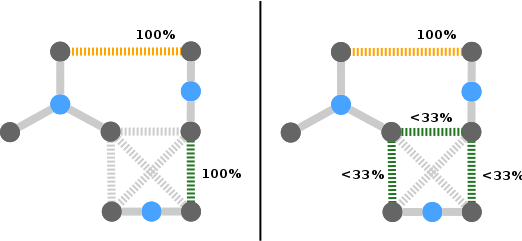
\includegraphics[width=0.56\textwidth]{figures/lessismore}%
	\caption{Due to the channel separation and exclusive access to one channel the left scenario is more favourable than the right, since throughput empirically
	exponentially decreases and is far below the 33 percent which those links would have to yield in order to at least provide the same throughput}
      }
      \label{fig:lessismore}
    \end{figure}
    In addition having some radio modules to spare gives us the opportunity to use those for client connections and assigning them a channel which does not interfere with the
    wireless backbone.
    \begin{figure}[h]
      \centerline{
	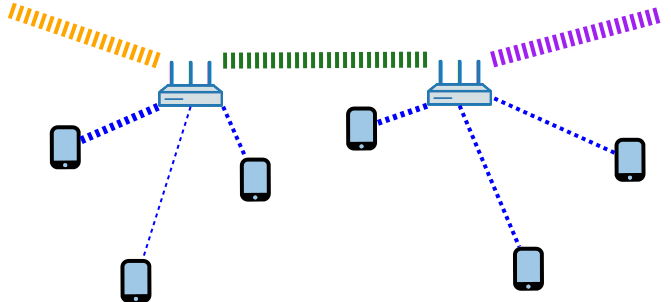
\includegraphics[width=0.56\textwidth]{figures/moduletospare}%
	\caption{Unused Modules used for separate client connections without interfering wlan backbone}
      }
      \label{fig:moduletospare}
    \end{figure}
  \subsection{Solution Works Within the Perimeter}
    The requirement dictates that computing a solution should be possible on a centralized entity (Servers/WLC).
    Our algorithm was implemented as a python script and can be run on a single system if given the right input data.
    Also the second requirement is fullfilled, since our algorithm is specially designed for a static environment where link quality and linkstate stay the same
    for a foreseeable time. If major changes in network connectivity or link quality occur the chosen network topology and channel assignment
    may lead to suboptimal results, therefore also a recomputation of the network topology has to be triggered.
    Currently there are no automatic triggers implemented, but planned in the future.
  \subsection{Comply with Economic Restrictions}
    The Runtime of the algorithms is mainly dependent on the number of connections between the nodes. Calculating the initial spanning tree is done in BFS mode and 
    therefore has quadratic runtime for the worst cast, depending on how sparse the graph is. The following calculation of the survival paths has also quadratic runtime 
    since we iterate over all connections and for each connection in the worst case over all other connections to find the backup path. The channel assignment is then again
    In a common deployment scenario the underlying network graph will be very sparsly connected since the number of accesspoints used and placement are carefully selected.
    Mostly they are placed in a way that they span a network over an area as far as possible.
    Current deployments and deployments in near future won't exceed 100 accesspoints. Even if fully meshed with a total of \(\sum \limits_{i=1}^{100} i = \frac{100(100+1)}{2}=5050\)
    edges it won't pose a problem to the capabilities of a WLC or an administrators machine.
  \subsection{Utilize Variable Number of Radios}
    As requested our algorithm selects channels from a given input set of channels. Only those channels are then used to determine the channel assignment.
    It is even possible to specify only one channel, resulting in a topology optimized network graph only.
\section{Reflection on Related Work}
  Comparing our solution to those of others would need some common ground. For example hardware requirements, number of modules and in general heterogenity/homgenity of
  the network are factor that could play in favor of some algorithms and therefore won't lead to fair results. Additionally different solutions were designed to 
  achieve different goals like throughput, latency or weighted throughput networks. Certainly there we could agree on this common deployment and compare each solution for random
  networks with respect to throughput, but this would require a full-scale simulation as hardware-resources are limited and too easily prone to real world difficulties.
  Although maybe a key aspect of this work, we did not have enough time to simulate even our own solution and therefore neither those of others. Nevertheless we would appreciate
  if someone further work on this field. In order to at least provide some kind of comparison we take a look at the features of each solution.
  \subsection{Features of Related Work Systems}
    TODO:
  \subsection{Features of Our System}
    TODO:
    
\section{Discussion}
  \begin{description}
   \item [Checking the coloring and channel assignment after the algo run]
   this might not be the best place for this point, but serves just as a reminder.
   \item [What do the results mean?]
   Obviously it is useful to use mutliple channels for WDS system
   \item[What could'nt we measure?]
   What measurements are still missing:  run testcases for each parameter like formula,...
   Evaluate the redundant paths feature.
   Simulate the system with more accesspoints and various parameteres
  \end{description}